
%\chapter{モンテスキュー}

\chapter{18世紀啓蒙主義}



\section{モンテスキュー『法の精神』(1748)}



典拠:モンテスキュー(1989)『法の精神』(上・中・下)、野田良之・稲本洋之助・上原行雄・田中治男・三辺博之・横田地弘訳、岩波書店





 % \begin{wrapfigure}{r}{60mm}
 %   \begin{center}
 %     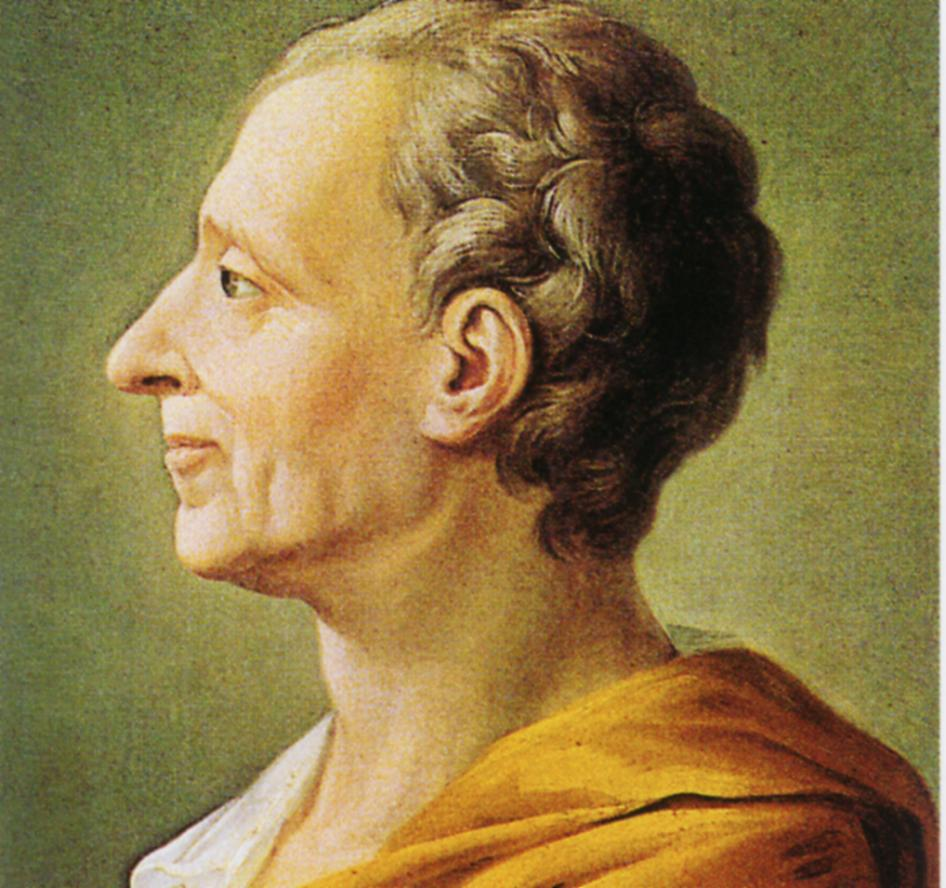
\includegraphics[width=50mm]{images/montesquieu.jpg}
 %     \caption{モンテスキュー} 
 %   \end{center}
 % \end{wrapfigure}


\subsection{}


法律とは、その最も広い意味では、事物の本姓に由来する必然的な諸関係である。そして、この意味では、ありとあらゆる存在はその法律をもっている。神はその法律をもち、物質的世界はその法律をもち、人間より上位の叡知的存在はその法律をもち、動物はその法律をもち、人間はその法律をもつ。

ある盲目的な宿命がこの世でわれわれが見るすべての結果を生み出した、と言った人々ははなはだしく不条理なことを言ったものである。なぜなら、盲目的な宿命が叡知的な存在を生み出したということ以上にはなはだしく不条理なことはありえまいと思われるからである。

したがって、一つの原始的理性が存在しているのであり、もろもろの法律は、この原始理性とさまざまな存在との間にある諸関係であり、また、これらのさまざまな存在相互間における諸関係なのである。(上・39-40)

\subsection{}


法律は、一般的には、それが地上のありとあらゆる人民を支配するかぎりにおいて、人間理性である。そして、各国民の国制の法律および公民の法律は、その人間理性が適用される特殊な場合にすぎないということでなければならない。

それらの法律は、その作られた目的たる人民に固有のものであるべきで、一国民の法律が他国民にも適合しうるというようなことは全くの偶然であるというほどでなければならない。
それらの法律は、国制の法律のように政体を形成するものであるにせよ、あるいは、公民の法律のようにそれを維持するものであるにせよ、すでに確立されている、あるいは確立されようとしている政体の本性と原理とに関係しなければならない。

それらの法律は、その国の自然的なるもの、すなわち、寒いとか、暑いとか、あるいは、温いとかの気候に、土地の質、位置、大きさに、農耕民族、狩猟民族、遊牧民族といった民族の生活様式に相関的でなければならない。それらの法律は、国制〔コンスティテュシオン〕が容認しうる自由の程度に、住民の宗教に、その性向に、その富に、その数に、その商業に、その習俗に、その生活態度に関係していなければならない。最後に、それらの法律は、それら相互間において関係をもつ。それらは、その起源、立法者の目的、その確立の基礎たる事物の秩序とも関係をもつ。まさにこれらすべてを見渡して、それらの法律を考察しなければならないのである。

私がこの著作においてなそうとするのは、以上のことである。私はこれらすべての関係を検討するであろう。これらの関係がすべて一緒になって「法律の精神」(esprit des lois)と呼ばれるものを形成する。(上・48-49)


 \begin{figure}[htbp]
   \centering
     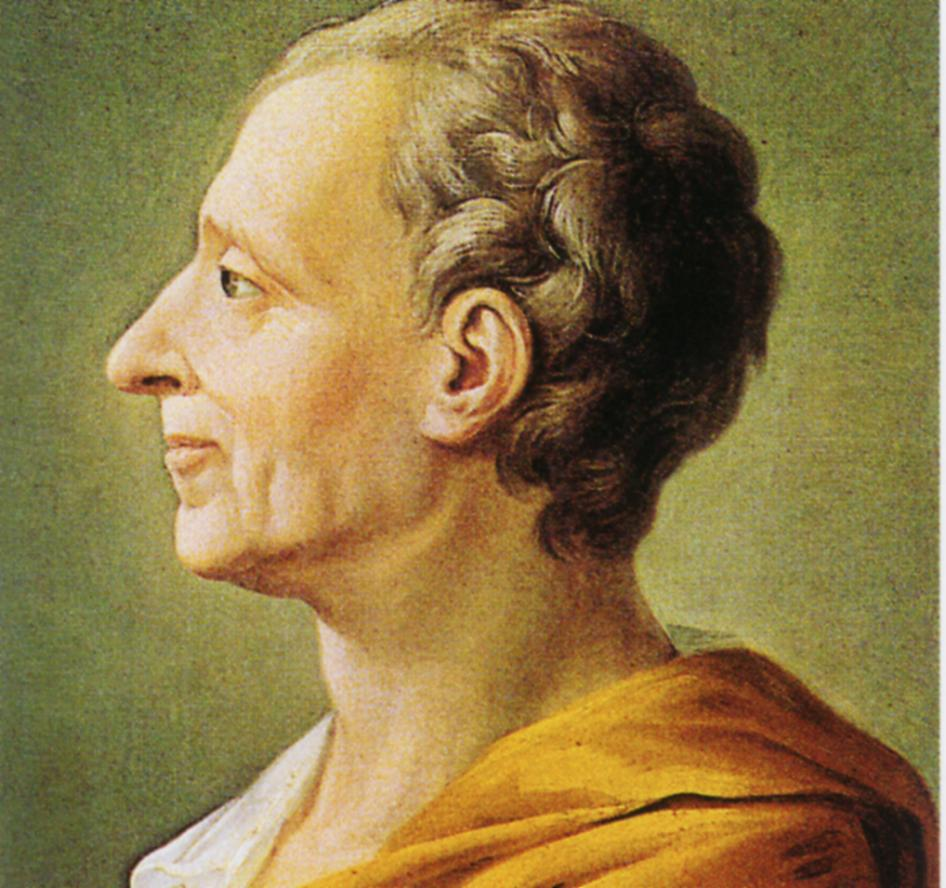
\includegraphics[width=50mm]{images/montesquieu.jpg}
   \caption{モンテスキュー}
 \end{figure}


\subsection{}



君主政体や専制政体が維持または持続されるためには、誠実さはあまり必要でない。前者においては法律の力が、後者においては君公の常に振り上げられた腕が、万事を規制かつ抑制する。しかし、民衆国会においては、もう一つのバネが必要であり、それは「徳」である。

私の言うところは、歴史の全体によって確認され、また事物の本性によく一致する。なぜなら、法律を執行させる者がみずからは法律の上位にあると思っている君主政においては、法律を執行させる者が彼自身法律の下位にあり、その重荷を背負うだろうと感じている民主政体においてよりも、徳の必要が少ないということは明らかだからである。

さらに、君主は誤った助言や怠慢のために法律を執行させることを中途でやめ、容易にその誤りを償うことができることもまた明らかである。彼は顧問会議を更迭したり、そうした怠慢自体を自分で改めさえすればよい。ところが、民主政体においては、法律が執行されなくなったときは、このことは共和政の腐敗からしか生じえないのであるから、国家はすでに滅亡しているのである。

前世紀において、イギリス人は彼らの間に民主政を確立しようとして甲斐のない努力をしたが、これはかなり見事な光景であった。事件に関与した連中は全く徳をもたなかったし、彼らの野心は一番思いきって事を行なった人の成功に刺激されていたし、ある党派の精神は他の党派の精神によってしか抑えられなかったという有様だったので、政体はたえず変っていた。人民は驚いて民主政を探し求めたが、どこにもそれを見出せなかった。結局、多くの変動や衝突や動揺の後、かつて排斥した当の政体に落ち着くほかはなかった。(上・71-72)

\subsection{}


民主政の原理は、人は平等の精神を失うときのみならず、極端な平等の精神をもち、各人が自分に命令するものとして選んだ人たちと平等でありたいと欲するときに腐敗する。その場合には、人民はみずからが委託した権力にすら我慢ができず、すべてを自分自身で行ない、元老院に代って審議し、役職者に代って執行し、すべての裁判役にとって代ろうと欲する。

共和政においては徳がもはや存在しえなくなる。人民が役職者の職務を行なうことを欲する。だから、人は役職者をもはや尊敬しない。元老院の審議はもはや重きをなさない。だから、人はもはや元老院議員に対して敬意をもたず、したがって、老人に対して敬意をもたない。老人を尊敬しないとなると、人は父親をも尊敬しなくなるであろう。夫も敬服に値せず、主人も服従に値しないだろう。すべての人がこうした放逸を愛するにいたり、命令の苦痛は、服従の苦痛と同様に重荷になるであろう。妻や子や奴隷は誰にも服従しないであろう。もはや習俗も、秩序への愛も存在せず、ついには徳も存在しなくなるであろう。(上・223-224)

\subsection{}



各国家には三種の権力、つまり、立法権力(la puissance législative)、万民法に属する事項の執行権力および公民法に属する事項の執行権力がある。

第一の権力によって、君公または役人は一時的もしくは永続的に法律を定め、また、すでに作られている法律を修正もしくは廃止する。第二の権力によって、彼は講和または戦争をし、外交使節を派遣または接受し、安全を確立し、侵略を予防する。第三の権力によって、彼は犯罪を罰し、あるいは、諸個人間の紛争を裁く。この最後の権力を人は裁判権力(la puissance de juger)と呼び、他の執行権力を単に国家の執行権力(la puissance exécutrice)と呼ぶであろう。

公民における政治的自由とは、各人が自己の安全についてもつ確信から生ずる精神の静穏である。そして、この自由を得るためには、公民が他の公民を恐れることのありえないような政体にしなければならない。

同一の人間あるいは同一の役職者団体において立法権力と執行権力とが結合されるとき、暴君的にそれを執行する恐れがありうるからである。

裁判権力が立法権力や執行権力と分離されていなければ、自由はやはり存在しない。もしこの権力が立法権力と結合されれば、公民の生命と自由に関する権力は恣意的となろう。なぜなら、裁判役が立法者となるからである。もしこの権力が執行権力と結合されれば、裁判役は圧制者の力をもちうるであろう。

もしも同一の人間、または、貴族もしくは人民の有力者の同一の団体が、これらの三つの権力、すなわち、法律を作る権力、公的な決定を執行する権力、犯罪や個人間の紛争を裁判する権力を行使するならば、すべては失われるであろう。(上・291-292)

\subsection{}


酒が風土に反しており、したがって健康にも反しているところでは、過度の飲酒が、個人によって悪しき結果をほとんど生まず、社会にとっても害悪がほとんどなく、飲酒癖が人々をただ愚劣にするだけで、凶暴にするようなことのない国々におけるよりも、いっそう厳しく罰せられるのは当然である。こうしたわけで、酔っぱらいを、彼の犯した過失のゆえにせよ、酩酊そのことのゆえにせよ処罰してきた法律は、個人の飲酒癖にのみ適用されたのであって、国民の飲酒癖には適用がなかった。ドイツ人は習慣で飲み、イスパニア人は気分で飲む。

暑い国々においては、繊維の弛緩が水分を多量に発散させる。しかし、固形部分はそれほど拡散しない。非常に微弱な活動しかせず、ほとんど弾性をもたない繊維は、消耗し切ることがほとんどない。そこで、それを回復させるためにはわずかの滋養液で十分である。それゆえ、暑い国々では、人はほんの少量の食事しかとらない。

種々の異なる風土の中には、種々の異なる生活様式を形成してきた種々の異なる必要が存在している。そして、これら種々の異なる生活様式が多様な種類の法律を形成してきたのである。ある一つの国において、人びとの間の交渉が多い場合には、ある種の法律が必要である。そういう交渉が全くみられない国民においては、別の法律が必要である。(中・40-41)

\subsection{}


数多くの事柄が人間を支配している。風土、宗教、法律、統治の格律、過去の事物の例、習俗、生活様式。こうしたものから、その結果である一般精神が形成されるのである。

各国民の中で、これらの原因の一つがより大きな力をもって作用するにつれて、他の原因はそれだけその一つの原因に譲歩する。自然と風土はほとんどそれだけで未開人を支配している。生活様式は中国人を拘束している。法律は日本で暴威を振っている。習俗はかつてスパルタにおいて範をなした。統治の格律と古来の習俗とはローマにおいて範をなした。(中・158)


\subsection{}


もし世界に、社交的気質、開かれた心、生の楽しみ、よき趣味、自分の思想を伝える容易さを具えた国民、生き生きとして気持ちのよい、ときには軽率で、しばしば無遠慮であるが、それとともに、勇気、寛大さ、率直さ、一定度の名誉心をもった国民があるとするなら、その徳性をさまたげないためには、法律によってその生活様式を阻害しようとつとめるようなことがあってはならないであろう。一般に性格が善良であるならば、そこに見出される若干の欠点のなにが問題になるだろうか。

ここで、女性を抑制し、彼女らの習俗を矯正するための法律を作り、彼女らの奢侈を制限することもできるであろう。しかし、それによって、この国民の富の源泉となっているある種の良き趣味、この国に外国人を惹きつけている慇懃さが失われることにならないかどうか誰が知りえようか。

国民の精神が政治の諸原則に反していないとき、それに従うべきなのは立法者の方である。なぜなら、われわれは、自由に、しかもわれわれの生来の天分に従って作り上げたもの以上によいものを作り出すことはないからである。

本性的に快活な国民に衒学的精神を与えても、国民は内に対しても外に対しても何物も得るところはないであろう。こうした国民には、軽薄な事柄を真面目に、真面目な事柄を快活にやらせておくがよい。(中・158-159)

\pagebreak{}



\section{ルソー『エミール』(1762)}



典拠:ルソー、今野一雄訳(1962-64)『エミール』(上)(中)(下)、岩波書店

\subsection{}



万物をつくる者の手をはなれるときすべてはよいものであるが、人間の手にうつるとすべてが悪くなる。人間はある土地にほかの土地の産物をつくらせたり、ある木にほかの木の実をならせたりする。風土、環境、季節をごちゃまぜにする。犬、馬、奴隷をかたわにする。すべてのものをひっくりかえし、すべてのものの形を変える。人間はみにくいもの、怪物を好む。なにひとつ自然がつくったままにしておかない。人間そのものさえそうだ。人間も乗馬のように調教しなければならない。庭木みたいに、好きなようにねじまげなければならない。

しかし、そういうことがなければ、すべてはもっと悪くなるのであって、わたしたち人間は中途半端にされることを望まない。こんにちのような状態にあっては、生まれたときから他の人々のなかにほうりだされている人間は、だれよりもゆがんだ人間になるだろう。偏見、権威、必然、実例、わたしたちをおさえつけているいっさいの社会制度がその人の自然をしめころし、そのかわりに、なんにももたらさないことになるだろう。自然はたまたま道のまんなかに生えた小さな木のように、通行人に踏みつけられ、あらゆる方向に折り曲げられて、まもなく枯れてしまうだろう。〔……〕

植物は栽培によってつくられ、人間は教育によってつくられる。かりに人間が大きく力づよく生まれたとしても、その体と力をもちいることを学ぶまでは、それは人間にとってなんの役にも立つまい。かえってそれは有害なものとなる。ほかの人がかれを助けようと思わなくなるからだ。そして、ほうりだされたままのその人間は、自分になにが必要か知るまえに、必要なものが欠乏して死んでしまうだろう。人は子どもの状態をあわれむ。人間がはじめ子どもでなかったなら、人類はとうの昔に滅びてしまったにちがいない、ということがわからないのだ。

わたしたちは弱い者として生まれる。わたしたちには力が必要だ。わたしたちはなにももたずに生まれる。わたしたちには助けが必要だ。わたしたちは分別をもたずに生まれる。わたしたちには判断力が必要だ。生まれたときにわたしたちがもってなかったもので、大人になって必要となるものは、すべて教育によってあたえられる。(上・23-24)

\subsection{}


自然は子どもが大人になるまえに子どもであることを望んでいる。この順序をひっくりかえそうとすると、成熟してもいない、味わいもない、そしてすぐに腐ってしまう速成の果実を結ばせることになる。わたしたちは若い博士と老いこんだ子どもをあたえられることになる。子どもには特有のものの見方、考え方、感じ方がある。そのかわりにわたしたちの流儀を押しつけることくらい無分別なことはない。そしてわたしは、十歳の子どもに判断力があるなら、身の丈も五尺くらいあっていいのではないかと思う。じっさい、そんな年ごろの子どもに理性がなんの役に立つというのか。理性は力のブレーキとなるものだが、子どもはそういうブレーキを必要としていない。(上・125-126)

\subsection{}



わたしたちは、いわば、二回この世に生まれる。一回目は存在するために。二回目は生きるために。はじめは人間に生まれ、つぎには男性か女性に生まれる。女を未完成の男と考える人たちはたしかにまちがっている。けれども外見的な類似を考えればそれは正しい。思春期にいたるまでは、男の子も女の子も、見たところ全然ちがわない。同じ顔だち、姿、顔色、声、なにもかも同じだ。女の子も子どもだし、男の子も子どもだ。こんなによく似ている生きものは同じ名称で呼んでさしつかえない。その後も性の発達をさまたげられている男性は一生のあいだそういう類似をもちつづける。かれらはいつまでたっても大きな子どもなのだが、女性は、そういう類似を失うことがないので、多くの点において、けっして子どもとは別のものにならないようにみえる。

しかし男性は、一般に、いつまでも子どもの状態にとどまっているようにつくられてはいない。自然によって定められた時期にそこからぬけだす。そして、この危機の時代は、かなり短いとはいえ、長く将来に影響をおよぼす。

暴風雨〔あらし〕に先だってはやくから海が荒れさわぐように、この危険な変化は、あらわれはじめた情念のつぶやきによって予告される。にぶい音をたてて醗酵しているものが危険の近づきつつあることを警告する。気分の変化、たびたびの興奮、たえまない精神の動揺が子どもをほとんど手におえなくする。まえには素直に従っていた人の声も子どもには聞こえなくなる。それは熱病にかかったライオンのようなものだ。子どもは指導者をみとめず、指導されることを欲しなくなる。(中・5-6)

\subsection{}



わたしのエミールは、いままでは自分のことしか考えていなかったが、かれと同じ人間に注目するようになると、すぐに自分をかれらにくらべてみることになる。そして、この比較がかれのうちに呼び起こす最初の感情は、第一位を占めたいということだ。これは自分にたいする愛が自尊心に変わる地点、そしてそれに関係するあらゆる情念があらわれてくる地点だ。けれども、そういう情念のなかでかれの性格において支配的になるのが人間的なやさしい情念であるか、それとも、残酷でよくない情念であるか、好意と同情にみちた情念であるか、それとも、人をうらやみ、人のものをほしがるような情念であるか、それを決定するには、人々のなかで自分はどういう地位にあるとかれは感じるか、また、かれが獲得したいと思っている地位に到達するためにどんな種類の障害を克服しなければならないと考えることになるか、それを知る必要がある。

その地位の獲得をめざすかれを導いていくために、人間の共通の偶有性によって人々の姿を示してやったのちに、こんどは、たがいにちがう点によって人々の姿を示してやらなければならない。ここで、自然的な、また社会的な不平等の程度が示され、社会秩序全体の一覧表が示されることになる。

人間を通して社会を、社会を通して人間を研究しなければならない。政治学と倫理学を別々にとりあつかおうとする人々は、そのどちらにおいてもなにひとつ理解しないことになるのだ。まず原始的な関係に注目して、どうして人間はその影響をうけなければならないか、そして、そこからどういう情念が生まれてくるかをみる。逆に、情念が発達することによってその関係が複雑になり、緊密になることがわかる。人間を自由独立にするのは腕力ではなく、むしろ節度をわきまえた心である。少数のものにしか欲望を感じない人は少数の人にしか執着をもたない。ところが、わたしたちの無益な欲望を肉体的な必要とたえず混同しながら、肉体的な必要を人間社会の基礎としている人々はいつも結果を原因と考え、かれらのあらゆる推論においてまちがってばかりいる。
自然の状態には現実的な事実にもとづく破棄することのできない平等がある。自然の状態にあっては人間同志のたんなるちがいが一方を他方に隷属させるほど大きいことはありえないのだ。社会状態には架空のむなしい権利の平等がある。この平等を維持するための手段そのものがそれをぶちこわしているのだ。そして、弱者を押さえつけるために強者にあたえられている国家権力は、自然が両者のあいだにおいた一種の均衡を破っているのだ。〔……〕(中・57-58)

\subsection{}



両性の相互的な義務のきびしさは同じではないし、また同じではありえない。この点について男性は不公平な差別をしていると女性が不平をいうとしたら、女性はまちがっている。この差別は人間がつくりあげたものではない。あるいはとにかく、それは偏見がつくりだしたものではなく、理性がつくったものだ。両性のうち、自然から子どもという預かりものを依託されている方は、他方にたいしてその責任をもたなければならない。もちろん、誓約を破ることはどちらにも許されていないし、女性のきびしい義務にたいするただ一つの報賞を妻にあたえようとしない不実な夫はすべて、正しくない残酷な男だ。けれども不貞の妻はそれ以上のことをする。そういう女は家族をばらばらにし、自然の絆をすべて断ち切るのだ。夫の子どもでない子どもを夫にあたえて、みんなをだまし、不貞をはたらいたうえにさらに裏切り行為に走るのだ。こういう罪悪はあらゆる混乱、あらゆる罪悪につながっているのではなかろうか。世にも恐ろしい状態があるというなら、自分の妻に信頼をもたず、このうえなくやさしい心の働きにも身をゆだねることのできないみじめな父親、わが子をだきしめながら、他人の子を、自分の不名誉の証拠となるものを、自分のほんとうの子の財産をうばいとる者を、だきしめているのではないかと疑惑を感じている不幸な父親の状態がそれだ。そんなことになったら、家庭というものはどうなるのか、罪ふかい妻のために、たがいに敵対しながら、愛し合っているようなふりをしなければならない、ひそかな敵の集まりになってしまうのではないか。

だから、妻は、忠実であるだけではなく、夫や身近な人たちから、すべての人から、忠実な妻だと考えられることが必要だ。つつしみぶかく、細心で、控え目にすることが、そして、自分の良心にたいしてと同じように、他人にたいしても、美徳のしるしを見せることが必要だ。とにかく、父親は、子どもを愛する必要があるというなら、子どもの母親を尊敬する必要がある。こういうわけで、見かけということさえ女性の義務の一つになるのであって、女性にとっては名誉とか評判とかいうことも、貞潔ということと同じように、欠くことのできないものになっている。こうした原則から、両性の道徳的な差別にともなって、義務とたしなみについての一つの新しい動機が生じ、それはとくに女性に、素行、態度、動作についてできるだけ細心の注意をはらうことを命じている。男女は平等だし、その義務も同じだ、などと大ざっぱなことを主張するのは、むなしいせりふをならべたてているだけのことで、右のようなことに答えられないかぎり、それはぜんぜん意味のないことだ。(下13-14)

\subsection{}


「わたしが市民の義務について語るとしたら、きみ〔=エミール〕はおそらく、どこに祖国があるのか、ときくだろう。そして、わたしをへこませたつもりでいるだろう。しかし、エミール、きみはまちがっていることになるだろう。祖国をもたない者にも、とにかく、国はあるからだ。やっぱり政府があり、見せかけだけでも法律があって、そのもとで人は平穏に暮らしてきたのだ。社会契約が守られたことはないとしても、一般意志がそうすべきだったように、個別的な利害がその人を保護してきたとしたら、かれが目のまえに見た悪行がよいことを好ませることになったとしたら、わたしたちの制度そのものがそれに固有の不正をかれに認識させ憎悪させることになったとしたら、それでもけっこうではないか。ああ、エミール、自分の国に負い目を感じない有徳な人間がどこにいるだろう。それがどんな国だろうと、人間にとってなにより大切なもの、その行動の道徳性と美徳にたいする愛を、かれはその国からうけているのだ。どこかの森の奥に生まれていたとしたら、かれはもっと幸福に、もっと自由に暮らしていられたかもしれない。しかし、なにものとも戦う必要を感じずに自分の傾向にしたがっていられるかれは、よき者であってもなんの功績ももたないことになったろう。有徳な人間にはなれなかったろう。ところがいまやかれは、自分の情念を克服して、有徳な人間になれるのだ。秩序の見せかけでもかれにその秩序を認識させ、好ませることになる。公共の福祉は、ほかのすべての者にとっては口実として役だつだけだが、かれにとっては現実の動機になる。かれは自分と戦い、自分を征服し、自分の利益を共同の利益のために犠牲にすることを学ぶ。かれは法律からなんの利益も得ていないというのは正しくない。法律は、悪い人間のあいだにあってさえ正しい人間としてふるまう勇気をかれにあたえている。法律はかれを自由にしてはくれなかったというのは正しくない。法律はかれに自分を支配することを教えたのだ。」(下・257-258)


\subsection{}

男と女は、性格においても、体質においても、同じようにつくられてはいないし、同じようにつくられるべきでもないということが証明されれば、男と女は同じ教育をうけるべきではないということになる。男と女とは、自然の指示にしたがって、協力して行動しなければならないが、同じことをなすべきではない。

……両性に共通にある能力も、すべてがどちらにも同じ程度にあたえられているわけではない。しかし、全体においてみれば、その差は相殺されている。女は女としてすぐれており、男と考えれば劣っている。女の権利を利用していれば、いつも女は有利な立場にある。男の権利を奪おうとすれば、かならず女は男よりも低いところにとどまる。……女性に男性の美点となることを学ばせ、女性に固有のものをなおざりにさせるのは、だから、明らかに女性の不利になるようにすることだ。

……だからといって、女性はどんなことについても無知でいるように育てるべきだ、ただ家事のつとめだけをさせておくべきだ、ということになるだろうか。男性は自分の妻を女中にすることになるのだろうか。……妻をまったくの自動機械にすることになるのだろうか。もちろん、そんなふうであってはならない。あんなに快い、あんなに微妙な才気を女性にあたえている自然は、そんなことを命じてはいない。はんたいに、自然は、考えること、判断すること、愛すること、知ること、顔と同じように精神をみがくこと、そういうことを女性に望んでいる。それらは女性に欠けている力の代わりになるように、そしてわたしたち男性の力を導くように、自然が与えている武器なのだ。女性は多くのことを学ばなけばならない。しかし、女性にふさわしい知識だけを学ぶべきだ。

……女性の教育はすべて男性に関連させて考えられなければならない。男性の気にいり、役に立ち、男性から愛され、尊敬され、男性が幼ないときは育て、大きくなれば世話をやき、助言をあたえ、なぐさめ、生活を楽しく快いものにしてやる、こういうことがあらゆる時代における女性の義務であり、女性に子供のころから教えなければならないことだ。


女性は男性を助ける役目を果すことが自然である。「女性の教育はすべて男性に関連させて考えられなければならない。男性の気に入り、役に立ち、男性から愛され、尊敬され、男性が幼いときは育て、大きくなれば世話をやき、助言を与え、なぐさめ、生活を楽しく快いものにしてる、こういうことがあらゆる時代における女性の義務であり、女性の子どものときから教えられなければならないことだ


……男性は外、女性は内、これこそ自然の法則である(下 21)

\newpage{}


\section{ベッカリーア『犯罪と刑罰』(1764)}

出典:ベッカリーア、『犯罪と刑罰』、風早八十二・五十嵐二葉訳、岩波書店(岩波文庫)、1959。


\subsection{序論から}


社会の利益はそのすべての成員に平等にわかたれなければならないはずだ。

それなのに、じっさいの人間の社会においては、あらゆる権力と幸福は特権的な小数者の上に、あらゆる弱さとみじめさを残る大多数の上に、集める傾向にある。

このような傾向は、すぐれた法律によってだけおさえることができる。だのに人間はふつう、もっとも大切なことがらを規定するほねおりをおしんで、これをいいかげんに時の解決にゆだね、あるいは最良の法律にそむくことに利益をもつような一部の人の思いのままにさせている。

……

歴史を開いてみよう。自由人どうしの間の自由な契約であるはずの法律というものが、じっさいにはほとんどつねに小数者の欲望の道具であるか、あるいは気まぐれな一時的必要から生れた産物でしかなく、人間性の賢明な観察者{\——}多数の人間の活動を「最大多数の最大幸福」という唯一最高の目的に導くことを知っている者{\——}によってつくられたものではないことがわかる。(19-20)

 \begin{figure}[htbp]
   \centering
     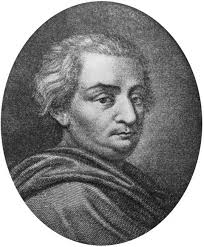
\includegraphics[width=50mm]{images/beccaria.jpg}
   \caption{ベッカリーア}
 \end{figure}


\subsection{}

……刑罰の起源はなにか? 刑罰権の基礎は何に求められるのだろうか? それぞれことなった犯罪に対して何が適当した刑罰だろうか? 死刑ははたして社会の安全と善良な秩序のために有用であり、欠くことのできない刑罰だろうか? 拷問や責め苦は正しいのか?また法律の要求する目的を達成させるものだろうか? 犯罪を予防する最良の方法は何か? 同じ刑罰があらゆる時代においてひとしく有用でありうるのか?それらの刑罰は風俗の上にどんな影響をおよぼすか?…… (23)

拘束されず孤立していた人間が、たがいに結合しあったその条件が法律をつくった。たえまない戦いの状態に疲れ、保持して行くことが不確実になったむなしい自由の享受に疲れた人間は、じぶんの自由の一部分をさし出して自由を確保することを考えたのである。この各人の自由の分け前の総和が一国の主権をかたちづくる。そして主権者とは、とりもなおさず、合法的にこれらの自由の供託を受け、その管理をおおせつかった者にほかならない。(25)

% この自由の小さな割り前の総和が刑罰権の基礎である。この基礎を逸脱する刑罰権の行使は、すべて濫用であり、不正である。それは事実上の権力ではあっても、法にもとづいた権利ではない。

刑罰が国民の一人に対する暴力行為にならないためには、それは本質的に公然、迅速、かつ必要なものでなければならず、与えられた一定の事情のもとで適用することができる刑罰のうちでもっとも軽くなければならず、また犯罪に比例した、法律によってはっきり規定されているものでなければなならない。

\subsection{拷問について}

いったい刑罰の目的はなにか? それは犯罪におもむこうとする他の人々の心にみせしめによってきざまれる威嚇である。

しかし拷問は{\——}圧政が、慣行的に、人目はなれた監房の中で犯人とおなじく無実の者にも加える、この秘密の責め苦は{\——}どう弁解できるのか?

もちろん、はっきりしているすべての犯罪が、不罰におわってはならないというのは大切なことである。しかし、不確実のやみにうずもれている犯罪の犯人をあばくということは、かならずしも有益なことではない。

すでに犯された犯罪で、もういまさら救済方法のないものは、つぎの目的のため以外に社会によって罰されるべきではない。すなわち不罰が、同じような犯罪を犯しても罰されないという希望を他の人々にもたせるばあいにかぎって、その希望をおいはらうために犯人を罰してよいのである。(60-61)

……われわれの意思行為は、その行為の原因となっている感覚におよぼす圧力に比例する。しかも人間の感受性には限度がある。だから苦痛の圧力が、被告の魂の根かぎりの力をくいつくしてしまうまで強まったとき、彼はその瞬間もう眼の前の苦痛からのがれるもっともてっとりばやい方法をとるしか考えなくなる。このようにして、被告の答弁は火や煮え湯が人間の皮膚に与える結果のように、必然の結果でしかない。

こうして責め苦に対する抵抗力の弱い無実の者は、自分は有罪だと自分で叫ぶのだ。そして、有罪の者と無実の者を見わけるためのその方法自体が、有罪と無実の区別を消してしまうのだ。(63)

\subsection{刑罰の緩和について}

% 刑罰が残酷になればなるだけ、{\——}いわば法律の残忍さの水準にしたがって{\——}人間の魂はかたくなになる。このようにすすんでいけば、

刑罰が残虐であればあるだけ、犯人は刑罰をのがれようとする。多くの犯罪はまさに、はじめの刑を逃がれようとしてかさねられたものなのだ。

おそろしい刑罰が習慣化されていた時代や国では、もっとも極道な犯罪も習慣化していた。

立法者に血の法律を示唆したその同じ気風が、暗殺者や親殺しの手に\ruby{匕首}{あいくち}を示唆したのだ。

葷酒は高い王座から鉄のムチのみによって治め、奴隷たちは圧政者を血祭りにあげ、それはまた新しい圧政者をみずからむかえる結果にしかならないのだった。(87-88)

\subsection{死刑について}

このように刑罰の責め苦を濫用することが決して人々を良くしないのを見て、私は検討したくなった。{\——}死刑はほんとうに有用なのか。賢明な政体にとって正しいことなのか。{\——}を。

人間が同胞を虐殺する「権利」を誰がいったい与えることができたのか? この権利はたしかに主権と法律との基礎になっている権利とは別のものだ。それは個々人の意思の総体である総意を表示する。さてしかし、誰が彼の生命をうばう「権利」を他の人々に与えたいなどと思っただろうか? どうして各人のさし出した最小の自由の割前の中に、生命の自由{\——}あらゆる財産の中でもっとも大きな財産である生命の自由もふくまれるという解釈ができるのだろう?

……

人間の精神にもっとも大きな効果を与えるのは刑罰の強度ではなくその継続性である。これはわれわれの感性が、はげしいが一時的な衝動によってより、よわいが持続的な印象によってずっとたやすくまた永続的な影響を受けるからである。……

この道理でいけば、犯罪への\ruby{轡}{くつわ}としては、一人の悪人の死は力よわいものでしかなく、強くながつづきのする印象を与えるのは自由を拘束された人間が家畜となりさがり、彼がかつて社会に与えた損害を身をもってつぐなっているその姿である。(91-93)

……死刑は見る者の大多数にとっては一つの見せ物でしかなく、のこりの少数の者にはいきどおりのまじった同情の対象となる。この二つの感じが見る者の心をすっかり占めてしまうから、死刑を規定する法律が目的とするような教訓的な恐怖などおしのけられてしまう。しかしより緩和されしかも持続的な刑罰は、これを見る者の心におそれだけをおぼえさせるのである。

……刑罰が正当であるためには、人々に犯罪を思いとどまらせるに十分なだけの厳格さをもてばいいのだ。そして犯罪から期待するいくらかの利得と、永久に自由を失うこととを比較判断できないような人間はいないだろう。

このようにして、死刑と置きかえられた終身隷役刑は、かたく犯罪を決意した人の心をひるがえさせるに十分なきびしさを持つのである。それどころか、死刑より確実な効果を生むものだとつけ加えたい。

……われあれの魂は、極度の苦痛であってもそれが一時的のものであれば比較的たえられる。むしろ、長い期間のたえまない不快にたえられないのである。なぜなら、一時的な苦痛に対しては、魂は全力を結集してそれをはねかえすが、長いたえまない苦しみに対抗していくためには魂の弾力性は十分ではないから。(94-95)

……

自らの無思慮の犠牲となった不幸な者たちによってあらわされるみせしめは死刑よりも強く人の心をうつ。死刑は人を矯正しないで、かえって人の心をかたくなにしてしまうが。

死刑はまた、人々に残酷行為の手本を与えるということで、もう一つ社会にとって有害だ。

たとえ、激情や戦争の必要性が人々に人類の血を流すことを教えるとしても、法律が、風紀を温和なものにすることを目的とする法律が、この野蛮行為をそれ以上ふやしていいものだろうか? …… 人殺しをいみきらい、人殺しを罰すう総意の表現にほかならない法律が、公然の殺人を命令する、国民に暗殺を思いとどまらせるために殺人をする{\——}なんとばかげていはしないか?(98-99)









\pagebreak{}


\section{スミス『国富論』(『諸国民の冨』)(1776)}


 % \begin{wrapfigure}{r}{60mm}
 %   \begin{center}
 %     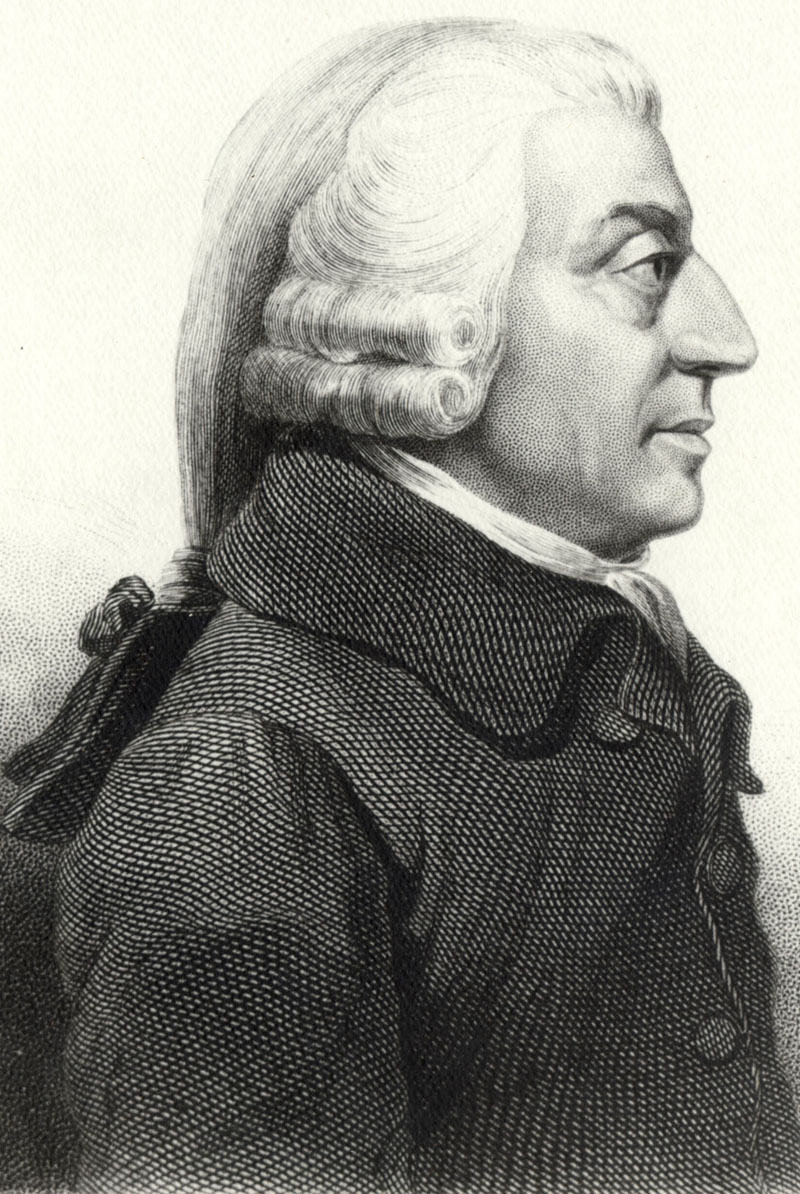
\includegraphics[width=50mm]{images/adamsmith.jpg}
 %     \caption{スミス} 
 %   \end{center}
 % \end{wrapfigure}


典拠:アダム・スミス、山岡洋一訳訳(2007)『国富論 上・下』日本経済新聞社


\subsection{}

労働の生産性が飛躍的に向上してきたのは分業の結果だし、各分野の労働で使われる技能や技術もかなりの部分、分業の結果、得られたものだと思える。

……きわめて小規模ではあるが、分業が注目されてきた産業を例にとってみよう。ピン、つまり裁縫用の待ち針を作る製造業の例である。ピンの製造は分業の結果、独立した職種になり、おそらくやはり分業の結果、専用の機器や道具が発明されてきたのだが、この職種の技能を身につけておらず、専用の機器や道具の使い方も知らない人なら、懸命に働いてもたぶん、一日に一本も作ることもできず、二十本を作ることはとてもできない。とこが現状をみると、ピン製造が一つの職種になっているうえ、いくつもの部門に分かれていて、そのかなりの部分がやはり独立した職種になっている。一人目が針金を引き伸ばし、二人目が真っ直ぐにし、三人目が切り、四人目が先をとがらせ、五人目が尖端を削って頭がつくようにする。頭を作るのも、二つか三つの作業に分かれている。頭をつけるのも一つの作業だし、ピンを磨いて光らせるおも一つの作業である。できがったピンを紙に包むことすら、一つの作業になっている。このようにして、留め針製造の仕事が十八ほどの作業に分かれている。十八の作業のすべてにそれぞれ人を割り当てている作業場もあるし、一人がといには二つか三つの作業をこなすようにしている作業場もある。わたしは小さなピン製造所をみたことがある。そこで働いていたのは十人なので、何人かは二つか三つの作業をこなしていた。とても貧しい作業場で、必要な機器も最低限のものしか揃っていなかったが、それでも懸命に働けば、一日に約十二ポンド(約5.4キロクグラム)を製造できた。1ポンドには、中型のピンなら4千本以上あるので、この十人で一日に4万8千本以上を製造でき、一人当りにすれば、一日に4千8百本を製造できる計算になる。……


ピンの製造はごく小さな産業だが、他の産業でも分業の効果はこれに似ているもっとも、たいていの産業では仕事をここまで細かく分けることはできず、作業をここまで単純にすることもできない。しかしどの産業でも、分業が可能であり実際に進んでいれば、その程度に応じて労働の生産性が向上している。(上・7-8)

……分業によって同じ人数が働いたときの生産性が大幅に増加するのは、三つの要因のためである。第一に、個々人の技能が向上する。第二に、一つの種類の作業から別の作業に移る際に必要な時間を節減できる。第三に、多数の機器が発明されて仕事が容易になり、時間を節減できるようになって、一人で何人分もの仕事ができるようになる。(上・10)


\subsection{}



ものを交換しあうこの性質が人間の本能の一つであって、それ以上の説明が不可能なものなのか、それとも、この方が正しいように思えるが、理性と言語という人間の能力によるものなのかは、ここで論じようとは思わない。この性質は人類に共通しており、他の種の動物にはみられない。動物は交換にかぎらず、どんな種類の約束や合意も知らないようだ。〔……〕二匹の犬がじっくりと考えたうえ、骨を公平に交換しあうのを見た人はいない。また、動物が仕草や鳴き声を使って、これは自分のもので、それはお前のものだ、これとそれを交換しようと仲間にもちかけるのを見た人もいない。動物が人や仲間の動物から何かをもらおうとするとき、分けてくれそうな相手に気に入られるようにする以外に方法はない。子犬は母犬にじゃれつくし、スパニエルは餌がほしいとき、食事中の飼い主の気をひくためにさまざまな芸をしてみせる。人間も同じ方法を使って他人の気をひこうとすることがある。自分が望むように行動してもらう方法が他にない場合、卑屈な態度をとって媚びへつらい、好意を得ようとする。しかし、毎回この方法をとろうとすると、時間がいくらあっても足りない。文明社会では、各人がいつでも無数の人の協力と助けを必要としており、そのうち一生の間に知りあえる人はごく一部にすぎないからだ。動物はほとんどの種で、それぞれの個体は成長すると独立し、自然の状態では他の生き物の助けを必要としない。しかし人はほぼいつでも他人の助けを必要としており、他人の善意だけに頼っていては、助けを得られると期待することはできない。相手の利己心に訴える方が、そして、自分が求めている行動をとれば相手にとって利益になることを示す方が、望みの結果を得られる可能性が高い。誰でも、取引をもちかけるときにはそのように提案している。わたしがほしいものをくれれば、希望するものをあげようというのが、そうした提案の意味なのだ。そして、人間はほとんどの場合、自分が必要とする他人の助けをこの方法で得ている。われわれが食事をできるのは、肉屋や酒屋やパン屋の主人が博愛心を発揮するからではなく、自分の利益を追求するからである。人は相手の善意に訴えるのではなく、利己心に訴えるのであり、自分が何を必要としているのかではなく、相手にとって何が利益になるのかを説明するのだ。主に他人の善意に頼ろうとするのは物乞いだけだ。しかし、その場合でも、他人の善意だけに頼っているわけではない。(上・16-17)

 \begin{figure}[htbp]
   \centering
     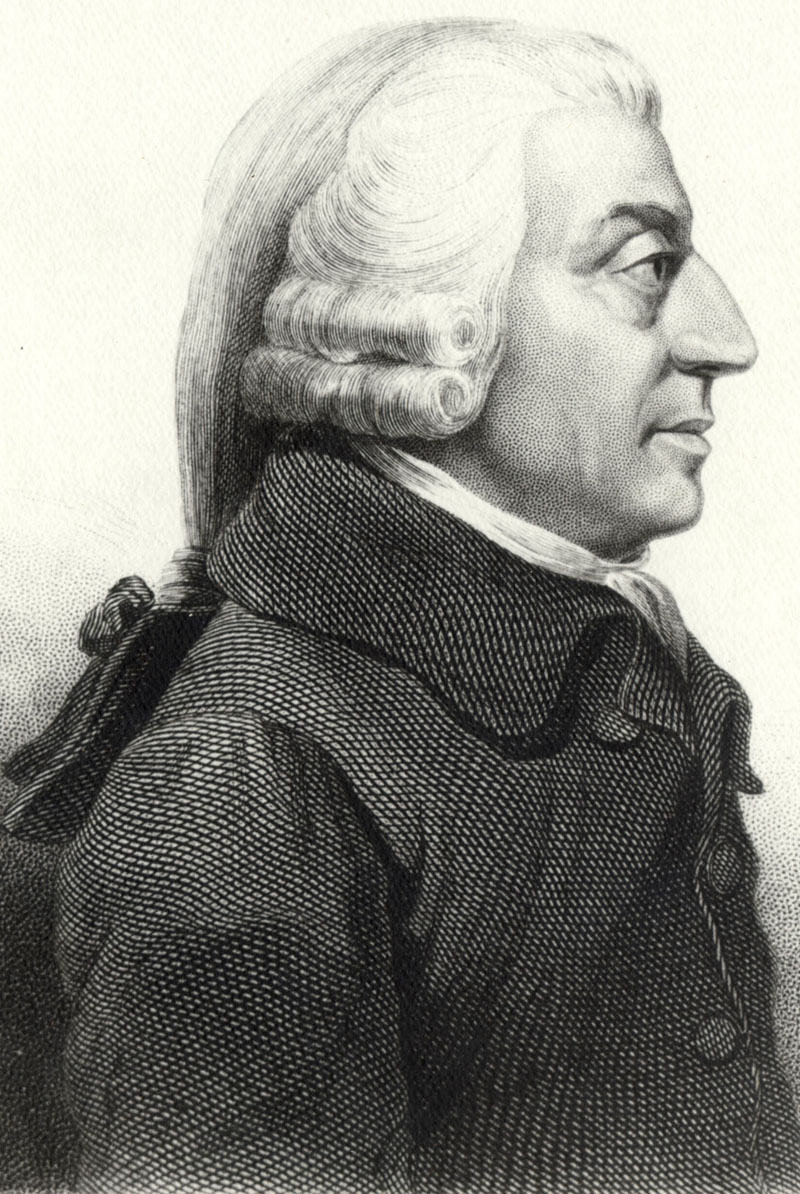
\includegraphics[width=50mm]{images/adamsmith.jpg}
     \caption{スミス} 
 \end{figure}


\subsection{}


分業が確立すると、各人が必要とするもののうち、自分の労働によって生産できる部分はごく一部にすぎなくなる。必要の大部分は、各人の生産物のうち自分で消費するもの以外の部分と交換して満たすようになる。全員が交換によって生活するようになり、ある意味で商人になる。社会全体も商業社会と呼べるものになる。

しかし、分業が起こりはじめた時点では、このような交換にかなりの障害があったはずだ。一方に、ある商品を自分が必要とする以上に持っている人がおり、他方に、それを持っていない人がいる状況を考えてみよう。この場合、一方は余った部分を手放そうとし、他方はそれを手に入れようとする。しかし、手放そうとする側がそのときに必要とするものを、手に入れようとする側がたまたま持っていなければ、交換は成立しない。たとえば肉屋が、自分が必要とする以上の肉を店に持っており、酒屋とパン屋がその一部を手に入れたがっているとする。酒屋もパン屋もそれぞれの仕事で生産したものしか持っておらず、肉屋が当面必要な量のビールとパンを持っていれば、互いの商品を交換することはできない。それぞれがあまり互いの役に立たない状態になる。このような状態から生まれる不便を避けるために、分業が確立した後、どの時代にも賢明な人はみな、自分の仕事で生産したもの以外に、他人が各位の生産物と交換するのを断らないと思える商品をある程度持っておく方法をとったはずである。(上・25-26)

\subsection{}



こうして、文明国のすべてで通貨が交換のための共通の手段になり、すべての種類の商品が通貨を使って売買され、交換されるようになった。

以下では、ものが売買され、交換されるときに、自然に守られる法則がどのようなものであるかを検討する。この法則によって、ものの相対価値とも交換価値とも呼ばれるものが決まる。

この「価値」という言葉に二つの意味があることに注意すべきだ。ときにはあるものがどこまで役立つか(どこまで効用があるか)を意味し、ときにはあるものを持っていることで他のものをどれだけ買えるかを意味する。この二つを「使用価値」と「交換価値」と呼ぶこともできる。使用価値がきわめて高いが、交換価値はほとんどないものも少なくない。逆に、交換価値がきわめて高いが、使用価値がほとんどないものも少なくない。水ほど役立つものはないが、水と交換して得られるものはほとんどない。これに対してダイヤモンドは、ほとんど何の役にも立たないが、それと交換してきわめて大量のものを得られることが多い。(上・30-31)

\subsection{}



どの商品でも加工段階が進むとともに、価格のうち賃金と利益にあてられる部分の比率が高くなり、地代にあてられる部分の比率が低くなる。加工段階が進むと、各段階での利益が積み重なっていくだけでなく、後の段階ほど前の段階より利益が多くなる。これは後の段階ほど、利益のもとになる資本が多くなるからである。たとえば、糸を紡ぐ紡績事業より、つぎの段階の織布事業の方が多額の資本を必要とする。織布事業では、糸を仕入れるときに紡績事業が資本を回収し利益を確保する価格を支払ったうえ、織工の賃金も支払うからであり、利益はかならず資本に比例するものだからである。
〔……〕

しかし、どの商品でも全価格が最終的に、この三つの部分のいずれかに、あるいは三つの部分のすべてにあてられている。土地の地代を払い、生産や製造、市場への輸送に使われた労働の賃金を支払った後に残るものがあれば、それは誰かの利益になるはずだからである。

個別の商品の価格、つまり交換価値は個々にみた場合、この三つの部分のいずれかに、あるいは三つの部分のすべてにあてられているのだから、ある国で一年間の労働によって生産される商品の価格も、全体としてみた場合、同じ三つの部分にあてられているはずであり、その国の住民の間に、労働の賃金、資本の利益、土地の地代のいずれかとして分配されるはずである。ある社会で一年間の労働によって生産されるもの、言い換えれば生産物の総額はまず、この三つの部分にあてられ、社会の構成員に分配される。賃金、利益、地代の三つがすべての収入の源泉であり、すべての交換価値の源泉である。その他の収入はすべて、最終的にこの三つの源泉のうちどれかに由来している。(上・54-55)

\subsection{}



社会全体の真の富が増加すれば、つまり、社会全体で有用な労働の量が増加すれば、土地の真の地代を間接的に上昇させる要因になる。有用な労働のうちある部分は当然、土地の生産物の生産に使われる。土地の耕作に使われる労働者と家畜が増え、生産に使われる資本が増加するとともに生産物が増加し、この増加に伴って地代が上昇する。

逆の状況になり、土地の耕作と改良が減るか、土地の生産物の一部で真の価格が低下するか、製造業が衰退して製品の真の価格が上昇するか、社会全体の真の富が減少すれば、どの場合にも土地の真の地代が下がり、地主の真の富が減少し、他人の労働かその生産物に対する地主の購買力が低下する。

どの国でも、土地と労働による年間の生産物、言い換えれば年間の総生産高は、前述のように、土地の地代、労働の賃金、資本の利益という三つの部分に自然に分配される。そして、地代で収入を得る地主、賃金で収入を得る労働者、利益で収入を得る資本家という三代階級の収入になる。これらがすべて文明社会で、基本的な構成要素になる三大階級であり、他の階級の収入はすべて、突きつめていけばこの三大階級の収入に由来している。(上・271-272)

\subsection{}



農村がまず発展してつぎに都市が発展するという順序は、すべての国にみられるわけではないが、一般論としては必要から生まれたものだし、それに、どの国でも人間の自然な好みによって刺激を受けている。人為的な制度によってこの自然な好みに沿った行動が妨げられなければ、都市はどの国でも、その国の土地の改良と耕作によって支えられる程度を超えて発展することはできない。少なくとも国内の土地がすべて完全に開発され、耕作されるまではそういえる。利益率が同じか、ほとんど変わらないのであれば、たいていの人は自分の資本の使い道として、製造業や貿易業よりも土地の改良と耕作を選ぶ。土地に資本を投じれば、貿易に資本を投じる場合よりも、事業を直接に監視し監督できるし、思わぬ出来事で資産を失うことも少ない。貿易業の場合には、風と波によって資産を失いかねない。それに、相手の人格や状況を熟知することがまずできないまま、遠くの国の商人に巨額の信用を与えるので、人間の愚かさと不誠実さというはるかに不確かな要因によっても資産を失いかねない。これに対して地主の資本は、土地改良に投じられており、世の中の性格を考えればこれ以上ないほど安全だと思える。そのうえ、農村は美しく、田舎暮らしは楽しく、心が落ちつくし、不当な法律によって妨げられないかぎり自主独立の立場を確立できるので、すべての人を多かれ少なかれひきつける魅力がある。そして、土地の耕作は人間にとって本来の仕事だったので、人類は歴史のどの段階にも、太古からの職業である農業を好む傾向をもちつづけているようだ。(上・391)

\subsection{}



ところで、どの社会でも年間の総収入はつねに、労働による年間の総生産物の交換価値に正確に一致する。というより、この交換価値とまったく同じものである。このため、各人が自分の資本をできるかぎり国内の労働を支えるために使い、しかも労働を生産物の価値がもっとも高くなるものに振り向けようと努力するのだから、各人はかならず、社会の年間の収入ができるかぎり多くなるように努力することになる。もっとも、各人が社会全体の利益のために努力しようと考えているわけではないし、自分の努力がどれほど社会のためになっているかを知っているわけでもない。外国の労働よりも自国の労働を支えることを選ぶのは、自分が安全に利益をあげられるようにするためにすぎない。生産物の価値がもっとも高くなるように労働を振り向けるのは、自分の利益を増やすことを意図しているからにすぎない。だがそれによって、その他の多くの場合と同じように、見えざる手に導かれて、自分がまったく意図していなかった目的を達成する動きを促進することになる。そして、この目的を各人がまったく意図していないのは、社会にとって悪いことだとはかぎらない。自分の利益を追求する方が、実際にそう意図している場合よりも効率的に、社会の利益を高められることが多いからだ。社会のために事業を行っている人が実際に大いに社会の役に立った話は、いまだかつて聞いたことがない。もっとも社会のためという考え方は、商人の間ではあまりみられないものなので、そのように考えるのをやめるべきだと説得するために言葉をつくす必要はない。(下・31-32)

\subsection{}



このように、各人は自己利益と好みとによって、通常の場合に社会にとってもっとも有利な用途に自分の資本を自然に振り向けようとする。だが、この自然な選考のために、そうした用途に振り向けられた資本が多すぎる状況になれば、その用途では利益率が低下し、他のすべての用途で逆に利益率が上昇して、各人はすぐに資本配分の間違いを改めようとする。したがって法律が介入しなければ、各人は自己利益と好みによって、社会全体の利益にもっとも適合したものにできるかぎり近い比率で、社会の総資本をその社会にあるすべての用途に自然に分配しようとするのである。

重商主義によるさまざまな規制はかならず、もっとも有利で自然な資本配分を多かれ少なかれ混乱させる。そして、アメリカ貿易とアジア貿易に関する規制はおそらく、他のどの規制よりも大きな混乱をもたらす。(下・218)

\subsection{}



以上から明らかなように、ある種類の産業を特別に奨励し、社会の資本のうちその産業で使われる部分の比率を自然に任せた場合より高めようとするか、ある種類の産業を特別に抑制し、社会の資本のうちその産業で使われる部分の比率を自然に任せた場合より低くしようとする政策はすべて、実際には、その政策の意図とは反対の結果をもたらす。こうした政策は真の富と偉大さに向けた社会の進歩を加速するのではなく、逆に妨げ、社会の土地と労働による年間生産物の真の価値を増やすのではなく、逆に減らすことになる。

ある産業を優遇するか抑制する制度をすべて完全に撤廃すれば、自然な自由という単純明快な仕組みが自然に確立する。誰でも、正義の法をおかさないかぎり、自分の利益を自分の方法で追求する完全な自由をもち、自分の資本と労働を使って誰とでも、どの階層とでも競争する完全な自由をもつようになる。こうなれば主権者は、民間人の労働を監視し、社会の利害という観点からもっとも適切な用途に振り向けようと試みる義務から解放される。この義務を遂行しようとすれば、主権者はいつも無数の錯覚に陥りかねず、人間の知恵や知識ではこの義務を適切に遂行することはできないのである。自然な自由の体制では、主権者が遂行しなければならない義務は三つしかない。この三つの義務はきわめて重要だが、単純明快であり、常識で理解できる。第一は、他国の暴力と侵略から時刻を守る義務である。第二は、社会の他の構成員による不正と抑圧から社会のすべての構成員を可能なかぎり守る義務、つまり厳正な司法制度を確立する義務である。第三は、ある種の公共施設を建設し、公共機関を設立して維持する義務である。この義務の対象になるのは、個人または少数の個人が建設・維持しても、その経費を回収できないので利益をあげることはできないが、社会全体にとっては、その経費を回収してもあまりあるほど有益なものである。(下・276-277)


第一編

労働の生産性の向上をもたらす要因と、各階層への生産物の分配にみられる自然の秩序

第二編

資本の性格、蓄積、利用

第三編

国による豊かさへの道筋の違い

第四編

経済政策の考え方

第五編

主権者または国の収入


労働には、対象物の価値を高めるものと、そのような効果がないものとがある。前者は価値を生み出すので、生産的労働と呼べるだろう。後者は非生産的労働と呼ばれるだろう(〔……〕)。製造工の労働は一般に、労働対象の原材料に、自分を維持する価値と、雇い主の利益になる価値とを付け加える。これに対して家事使用人の労働は、何にも価値を付け加えない。(上・338)


このように、資本と収入の比率がどこでも、勤勉な人と怠惰な人の比率を決めるようだ。資本が圧倒的な比率を占めるところではどこでも、勤勉な人が中心になる。収入が圧倒的な比率を占めるところではどこでも、怠惰な人が中心になる。このため、資本が増減すれば自然に、それに伴って生産的労働の実際の量、つまり生産的労働者の数が増減し、その結果、その国の土地と労働による生産物の交換価値、つまりその国の住民の真の富と収入が増減する。

資本は倹約によって増加し、浪費と無謀な経営によって減少する。(上・345)


\newpage{}
\section{カント「啓蒙とは何か』 (1784)}


\subsection{}



啓蒙とは、人間がみずから課した子ども状態から抜け出ることである。子ども状態とは、他人の指導なしには自分の悟性(理解力)を用いる能力がないことである。このような子ども状態の原因が悟性の欠如にではなく、他人の指導がなくとも自分の悟性を用いる決意と勇気の欠如にあるなら、子ども状態の責任は本人にある。「\emph{Sapere Aude!} あえて知ろうとせよ!/あえて賢くあれ!」「自分自身の\ruby{悟性}{あたま}を使う勇気を持て!」こそ啓蒙のモットーである。・・・未成年でいることは、たしかに気楽である。わたしのかわりの悟性をもつ本、わたしのかわりの良心をもつ牧師、わたしにかわって食事を気づかってくれる医者などがあれば、わたしはあえて自分の力を使う必要などない。支払うお金さえわたしにあれば、自分で考える必要などない。誰か他のひとがわたしのかわりに厄介なことを考えてくれるだろう。親切にも人々の後見を買って出ている保護者たちが、大多数の人々(これには女性全部が含まれる)が、成熟することを、難しいとだけでなく危険でもあると思いこむように仕組んでいるのである。まず自分の家畜たちを愚鈍にてなづけ、次にそうして従順になった家畜たちが、つなぎとめられている補助車なしには一歩も歩き出せないようにした上で、万が一、彼らが一人で歩きだそうとなどすれば、この保護者たちは危険だぞと怯えさせる。ところがこんな危険というものはたいしたものではない。なんどか転んでしまえば、けっきょくはちゃんと歩き方を学ぶことができるのだから。しかしこういった戒めでさえ、ひとびとを気おくれさせ、それ以上のことを試みなくさせるに十分なのである。



     \begin{figure}[htbp]
       \centering
         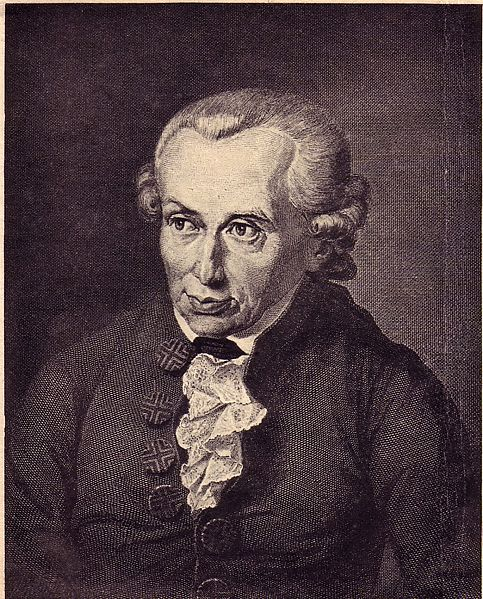
\includegraphics[width=50mm]{images/Kant.jpg}
       \caption{カント}
     \end{figure}



\section{カント『永遠平和のために』 (1795)}





典拠:カント、宇都宮芳明訳(2009)『永遠平和のために』岩波書店

\subsection{}


第二条項

独立しているいかなる国家(小国であろうと、大国であろうと、この場合問題ではない)も、継承、交換、買収、または贈与によって、ほかの国家がこれを取得できるということがあってはならない。

つまり国家は、(国家が場所を占めている土地のようなぐあいに)所有物(財産patrimonium)ではない。国家は、国家それ自身以外のなにものにも支配されたり、処理されたりしてはならない人間社会である。ところがそれ自身が幹として自分自身の根をもっている国家を、接ぎ枝としてほかの国家に接合することは、道徳的人格である国家の存在を廃棄し、道徳的人格を物件にしてしまうことで、したがってこうした接合は、民族についてのいかなる法もそれなしには考えられないような、根源的契約の理念に矛盾する。こうした取得方法についての誤った考え、つまり国家もまた互いに結婚できるといった考えは、ヨーロッパ以外のほかの諸大陸ではまったく知られなかった考えであるが、この考えが現代のわれわれにいたるまでヨーロッパにどれほどの危険をもたらしてきたかは、だれもがよく知っていることである。これは企業の新方式で、資力を費やさないで家族の縁組によって強力になる仕方であり、また同じ仕方で土地の所有を拡げるやり方である。{\——}また一国の軍隊をほかの国に貸し与え、共同の敵ではない第三国を攻撃するのに使用させるのも、この種の誤りに数えることができる。なぜなら、臣民はその際、任意に取り扱われるような物件として用いられ、消費されるからである。(15-16)

\subsection{}


第三条項

常備軍(miles perpetuus)は、時とともに全廃されなければならない。

なぜなら、常備軍はいつでも武装して出撃する準備を整えていることによって、ほかの諸国をたえず戦争の脅威にさらしているからである。常備軍が刺戟となって、たがいに無制限な軍備の拡大を競うようになると、それに費やされる軍事費の増大で、ついには平和の方が短期の戦争よりもいっそう重荷となり、この重荷を逃れるために、常備軍そのものが先制攻撃の原因となるのである。そのうえ、人を殺したり人に殺されたりするために雇われることは、人間がたんなる機械や道具としてほかのものの(国家の)手で使用されることを含んでいると思われるが、こうした使用は、われわれ自身の人格における人間性の権利とおよそ調和しないであろう。だが国民が自発的に一定期間にわたって武器使用を練習し、自分や祖国を外からの攻撃に対して防備することは、これとはまったく別の事柄である。{\——}財貨の蓄積も、同じ危険をもたらすであろうが、それは財貨がほかの国によって戦争の脅威とみなされ、その国の財貨の保有量をほかから探索する困難さが妨げとならないかぎり、ほかの国の先制攻撃を強いる原因となりかねないからである(なぜなら、\kenten{兵力}と\kenten{同盟力}と\kenten{金力}という三つの力のうち、金力がおそらくもっとも信頼できる戦争道具であろうから)。(16-17)


\subsection{}


第五条項

いかなる国家も、ほかの国家の体制や統治に、暴力をもって干渉してはならない。
なぜなら、いったいなにが国家にそうした干渉の権利を与えることができるというのであろうか。一国家が他国家の臣民たちに与える騒乱の種のたぐいがそれである、というのであろうか。だが一国家に生じた騒乱は、一民族が無法によって招いた大きな災厄の実例として、むしろ他民族にとって戒めとなるはずである。一般に、ある自由な人格が他の人格に悪い実例を示しても、それは(示された醜行scandalum acceptumとして)他の人格を傷つけることにはならない。{\——}もっとも、一つの国家が国内の不和によって二つの部分に分裂し、それぞれが個別に独立国家を称して、全体を支配しようとする場合は、事情は別かもしれない。その際、その一方に他国が援助を与えても、これはその国の体制への干渉とみなすことはできないだろう(その国はその時無政府状態にあるからである)。だがこうした内部の争いがまだ決着していないのに、外部の力が干渉するのは、内部の病気と格闘しているだけで、他国に依存しているわけではない一民族の権利を侵害するもので、児の干渉自体がその国を傷つける醜行であるし、あらゆる国家の自律を危うくするものであろう。(19-20)

\subsection{}



永遠平和のための第一確定条項

各国家における市民的体制は、共和制でなければならない。

第一に、社会の成員が(人間として)\kenten{自由}であるという原理、第二に、すべての成員が唯一で共同の立法に(臣民として)従属することの諸原則、第三に、すべての成員が(国民として)\kenten{平等}であるという法則、この三つに基づいて設立された体制{\——}これは根源的な契約の理念から生ずる唯一の体制であり、この理念に民族の合法的なすべての立法が基づいていなければならないのであるが、こうした体制が\kenten{共和的}である。それゆえ、この体制は、法にかんして、それ自体があらゆる種類の市民的組織の根源的な地盤となる体制である。そこで問題は、ただ次のこと、つまりこの体制がまた、永遠平和へと導くことができる唯一の体制なのか、ということである。

さて、共和的体制は、その根源が純粋であり、法概念の純粋な源泉から生じたものであるが、それだけではなく、さらに望ましい結果である永遠平和への期待にそった体制であって、その理由は次の点にある。{\——}すなわち、戦争をすべきかどうかを決定するために、国民の賛同が必要となる(この体制の下では、それ以外に決定の方途はないが)場合に、国民は戦争のあらゆる苦難を自分自身に背負いこむ(たとえば、自分で戦う、自分自身の財産から戦費を出す、戦争が残した荒廃をやっとの思いで復旧する、こうした災厄をさらに過重にするものとして、最後になお、平和であることすらも苦々しくさせるような、[たえず新たな戦争が近づいているために]決して完済にいたらない負債を自分に引き受ける、など)のを覚悟しなければならないから、こうした割りに合わない賭け事をはじめることにきわめて慎重になるのは、あまりにも当然のことなのである。これに反して、臣民が国民ではないような体制、つまり共和的ではない体制においては、戦争はまったく慎重さを必要としない世間事であるが、それは元首が国家の成員ではなくて、国家の所有者であるからである。かれは戦争によって、かれの食卓や狩りや離宮や宮中宴会などを失うことはまったくないし、そこで取るに足らない要因から戦争を一種の遊戯のように決定し、ただ体裁を整えるために、いつも待機している外交使臣団に戦争の正当化を適当にゆだねることができるのである。(33-34)

\subsection{}


永遠平和のための第二確定条項

国際法は、自由な諸国家の連合制度に基礎を置くべきである。

国家としてまとまっている民族は、個々の人間と同じように判断されてよい。つまり諸民族は、その自然状態においては(つまり外的法則に拘束されていない場合は)、隣りあっているだけですでに互いに害しあっているのであり、そこで各民族は自分たちの安全のために、それぞれの権利が保障される場として、市民的体制と類似した体制に一緒に入ることを他に対しても要求でき、また要求すべきなのである。これは\kenten{国際連合}と言えるが、しかしそれは当然諸民族連合一国家ではないであろう。そのような国家には、むしろ矛盾があることになろう。なぜなら、どの国家も\kenten{上位の者}(立法する者)の\kenten{下位の者}(服従する者、すなわち民族)に対する関係を含むが、もし多くの民族が一つの国家に吸収されると、ただ一つの民族しか形成しないことになって、これは前提に矛盾するからである(というのも、われわれはここでは\kenten{諸民族}相互間の法を考察しなければならないが、それはさまざまな民族がそれぞれ異なった国家を形成すべきで、一つの国家に融合すべきではないかぎりにおいてなのである)。(39-40)

\subsection{}



ところで、諸国家がそれぞれ自分の正義を主張する仕方は、当事者のほかに裁判所がある場合のように、審理という形をとることは不可能で、ただ戦争という形をとるほかない。だが戦争によって、しかもその幸運な結果である\kenten{勝利}によって、どちらが正義か決まるわけではなく、また\kenten{平和条約}によって、なるほど今回の戦争は終結するが、戦争状態(いつも新しい口実を見つけようとしている状態)は終結したわけではない(この状態がただちに不法であると宣告するわけにもいかないが、それはこの状態においては、それぞれの国家がめいめい自分の事柄にかんして裁判官だからである)。だがまた、無法な状態にあるある人間には、自然法によって、「この無法な状態から脱出すべきである」と言えるが、諸国家に対しては、これと同じことが国際法によって言えるわけではない(なぜなら、諸国家はそれぞれ国家として国内にすでに法的体制をもち、それゆえ諸国家が国家間の法概念にしたがって、さらに拡大された法的体制の下に入るべきだという他からの強制は、受け入れにくくなっているからである)。しかしそれにもかかわらず、理性は道徳的に立法する最高権力の座から、係争解決の手続きとしての戦争を断乎として処罰し、これに対して平和の状態を直接の義務とするが、それでもこの状態は、民族間の契約がなければ、樹立されることも、また保証されることもできないのである。{\——}以上に述べた諸理由から、\kenten{平和連合}(foedus pacificum)とでも名づけることができる特殊な連合が存在しなければならないが、これは\kenten{平和条約}(pactum pacis)とは別で、両者の区別は、後者がたんに\kenten{一つの}戦争の終結をめざすのに対して、前者は\kenten{すべての}戦争が永遠に終結するのをめざすことになる、と言えよう。この連合が求めるのは、なんらかの国家権力を手に入れることではなくて、もっぱらある国家そのもののための\kenten{自由}と、それと連合したほかの諸国家の\kenten{自由}とを維持し、保障することであって、しかも諸国家はそれだからといって、(自然状態にある人間のように)公法や公法の下での強制に服従する必要はないのである。{\——}\kenten{連合制度}は次第にすべての国家の上に拡がり、そうして永遠平和へと導くことになろうが、連合制度のこうした理念の実現可能性(客観的実在性)は、おのずから証明されるのである。なぜなら、もし幸運にもある強力で啓蒙された民族が一共和国(共和国は、その本性上、必然的に永遠平和を好むが)を形成することができたら、この共和国がほかの諸国家に対して連合的結合のかなめの役をはたすからで、その結果諸国家はこの結合に加盟し、こうして諸国家の自由な状態は国際法の理念に即して保障され、連合はこの種の多くの結合を通じて次第に遠くまで拡がっていくのである。(43-45)

\subsection{}



永遠平和のための第三確定条項

\kenten{世界市民法}は、普遍的な友好をもたらす諸条件に制限されなければならない。

ここでもまたこれまでの条項におけるのと同じように、問題とされているのは人間愛ではなく、\kenten{権利}であって、\kenten{友好}(よい待遇)と言っても、それは外国人が他国の土地に足をふみ入れても、それだけの理由でその国の人間から敵意をもって扱われることはない、という権利のことである。その国の人間は、外国人の死を招くような結果にならなければ、その人間を退去させることもできる。しかしその外国人が、他国の地で平和にふるまうかぎり、敵対的な扱いを受けることがあってはならない。だが外国人が要求できるのは、\kenten{客人の権利}(この権利を要求するには、かれを一定の期間家族の一員として扱うという、好意ある特別な契約が必要となろう)ではなくて、\kenten{訪問の権利}であるが、この権利は、地球の表面を共同に所有する権利に基づいて、たがいに交際を申し出ることができるといった、すべての人間に属している権利である。地球の表面は球面で、人間は地表の上を無限に分散していくことはできず、結局は並存して互いに忍耐しあわなければならないが、ところで人間はもともとだれひとりとして、地上のある場所にいることについて、他人よりも多くの権利を所有しているわけではない。{\——}この地表で住むことが不可能な部分、つまり大洋や砂漠は、こうした人間相互の交際を阻んでいるが、それでも\kenten{船}やラクダ(砂漠の\kenten{船})は、ひとびとがこの無主の地域をこえて互いに近づくことを可能にし、人類に共通に属している\kenten{地表}の権利を、生じてくる交際のために適用することを可能にしているのである。それゆえ、近海に近づく船を掠奪したり、漂着した船員を奴隷にするといった、海岸での(たとえばバーバリ地方の住民たちの)非道な扱いや、遊牧民族に近づくと、それをかれらを掠奪してよい権利とみなすような、砂漠での(アラビアのベドウィン人たちの)非道な扱いは、自然法に反している。とはいえ、こうした友好の権利、つまり外国人の権限は、原住民との交際を\kenten{試みる}ことを可能にする諸条件をこえてまで拡張されはしないのである。{\——}このような仕方で、遠く離れた諸大陸も互いに平和な関係を結び、この関係はついには公で法的なものとなり、こうして人類を結局は世界市民的体制へと次第に近づけることができるのである。(49-51)

\subsection{}


3 このように自然は、賢明にも諸民族を分離し、それぞれの国家の意志が、国際法を理由づけに用いながら、そのじつ策略と力によって諸民族を自分の下に統合しようとするのを防いでいるが、しかし自然は他方ではまた、互いの利己心を通じて諸民族を結合するのであって、実際世界市民法の概念だけでは、暴力や戦争に対して、諸民族の安全は保障されなかったであろう。\kenten{商業精神}は、戦争とは両立できないが、おそかれ早かれあらゆる民族を支配するようになるのは、この商業精神である。つまり国家権力の下にあるあらゆる力(手段)のなかで、\kenten{金力}ことはもっとも信頼できる力であろうから、そこで諸国家は、自分自身が(もとより道徳性の動機によるのではないが)高貴な平和を促進するように強いられ、また世界のどこででも戦争が勃発する恐れがあるときは、あたかもそのために恒久的な連合が結ばれているかのように、調停によって戦争を防止するように強いられている、と考えるのである。実際、戦争にむけての大合同は、事柄の本性から見てきわめてまれにしか生じないし、それが成功するのはさらにまれだからである。{\——}このような仕方で、自然は人間の傾向そのものにそなわる機構を通じて、永遠平和を保証する。なるほどこの保証は、永遠平和の到来を(理論的に)\kenten{予言する}のに十分な確実さはもたないけれども、しかし実践的見地では十分な確実さをもち、この(たんに空想的ではない)目的にむかって\kenten{努力する}ことをわれわれに義務づけるのである。(73-75)







\section{推薦図書}

\begin{itemize}
\item 作田啓一 (1980)『ジャン‐ジャック・ルソー:市民と個人』、人文書院。
\item 桑瀬章二郎 (2010)『ルソーを学ぶ人のために』、人文書院。定評ある「学ぶ人のために」シリーズの一冊。現代の研究動向がわかる。(渡)
\item 仲正昌樹 (2011) 『今こそルソーを読みなおす』、日本放送協会出版。わかりやすい良書。
\item 福鎌忠恕(1975)『モンテスキュー:生涯と思想』、酒井書店。全三冊の大作だが、時代背景の中でモンテスキューの思想形成を活写して読ませる。(渡)
\item 高島善哉 (1968) 『アダム・スミス』岩波書店〔岩波新書(青版)674〕
\item 山崎怜 (2005) 『アダム・スミス』、研究社出版。
\item 堂目卓生 (2008) 『アダム・スミス 『道徳感情論』と『国富論』の世界』、中央公論新社〔中公新書1936〕。新旧の定評ある新書。あわせて読めば日本の社会思想の変化も見える。(渡)
\item 
ハンナ・アーレント(1987)『カント政治哲学の講義』、浜田義文監訳、法政大学出版局。
\item 浜田義文 (編) (1989)『カント読本』、法政大学出版局。「学ぶ人のために」シリーズと並んで定評ある「読本」シリーズの一冊。20世紀の思想家による講義とあわせてどうぞ。(渡)
\end{itemize}


%%% Local Variables:
%%% mode: japanese-latex
%%% TeX-master: "main_gendai"
%%% coding: utf-8
%%% End:
